\section{Sensitivity Reach of B-factories from $e^+ e^-$ Annihilation}
For $e^+ e^-$ collisions, we make use of \madgraph again to handle our signal and background estimates.
Most of what was said about generation of events for the muon events holds here.

The total integrated luminosities at \belle is taken to be $1040.86fb^{-1}$, with \babar half this, and \belletwo to be expected to have around $100$ times this.
Since the centre of mass energy reaches $10.58\textrm{GeV}$, we can access the $\tau$ leptons here, which in our model have a very strong coupling to the scalar due to their large mass of $1.777\textrm{GeV}$.
There are two regions of interest in this scenario for the mass of the mediator: below, and above the threshold for the scalar to decay to muons.
Below this it can only decay to an $e^+ e^-$ pair, so the overall process for $m_\phi < 2m_\mu$ is

\begin{equation}
    e^+ + e^- \rightarrow \tau^+ + \tau^- + e^+ + e^-
\end{equation}

\noindent while above this threshold we decay almost exclusively to muons.

\begin{equation}
    e^+ + e^- \rightarrow \tau^+ + \tau^- + \mu^+ + \mu^-
\end{equation}

\subsection{Backgrounds}
Here we simply write down the irreducible SM background process, and let \madgraph run.
We generate $10,000$ background events for each of the two final states.
A sample Feynman diagram is shown in Fig.\ \ref{fig:ee_tautaull_SM}.

\begin{figure}[h]
    \centering
    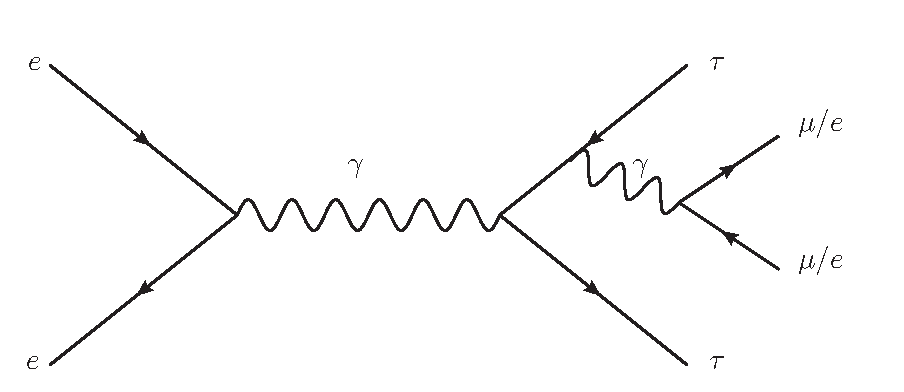
\includegraphics[width=0.6\textwidth]{Figures/feynman_diagrams/ee_tautaull_SM}
    \caption{One Feynman diagram for the background process $e^+ e^- \rightarrow \tau^+ \tau^- \ell^+ \ell^-$.}
    \label{fig:ee_tautaull_SM}
\end{figure}

\subsection{Signal}
Again, we simply define our process and let \madgraph run akin to the muon decay generation.
$10,000$ events are generated at each of $20$ mass points from $2m_e$ up to $2m_\mu$, and again from $2m_\mu$ up to $2m_\tau$.
However we do not go above $2m_\tau$ for simplicity, as this will open the $4\tau$ channel, whose signature does not have the advantage of being a spectrally peaked signal. 
We enforce that the generation of the scalar is once again on-shell, so our process is really the decay chain below.

\begin{equation}
    e^+ + e^- \rightarrow \tau^+ + \tau^- + \phi,~\phi \rightarrow \ell^+ + \ell^-
\end{equation}

A sample Feynman diagram for the signal is shown in Fig.\ \ref{fig:ee_tautaull_scalar}.

\begin{figure}[h]
    \centering
    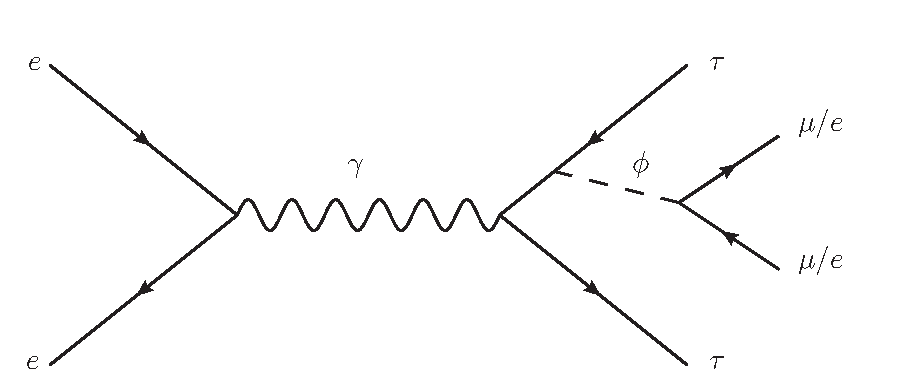
\includegraphics[width=0.6\textwidth]{Figures/feynman_diagrams/ee_tautaull_scalar}
    \caption{One Feynman diagram for the signal process $e^+ e^- \rightarrow \tau^+ \tau^- \ell^+ \ell^-$. The scalar must live on-shell before decaying promptly to a pair of leptons.}
    \label{fig:ee_tautaull_scalar}
\end{figure}

For our signal, since this is now a collision scenario and not a decay, we must weight our total number of events by the cross section determined by \madgraph.
The width we have chosen here is also just the energy resolution of the detector listed in the technical design report for \belletwo \cite{Abe:2010gxa} as

\begin{equation}
    \frac{\sigma_E}{E} = \sqrt{\left(\frac{0.066\%}{E}\right)^2 + \left(\frac{0.81\%}{E^{1/4}}\right)^2 + \left(1.34\%\right)^2}
\end{equation}

\noindent with $E$ being measured in $\textrm{GeV}$.

One of the more interesting components to this signal, is that we do not need to fully reconstruct both outgoing $\tau$ particles.
It is sufficient that we have one of them decay leptonically, $\tau^- \rightarrow \ell^- \bar{\nu}_\ell \nu_\tau$ (or the conjugate decay), which comes with a total branching fraction $\textrm{BR} = 0.1742 + 0.1783 = 0.3524$ \cite{Agashe:2014kda}.
For the other $\tau$, we allow all decay modes.
Thus, our signal really is three charged leptons in the final state, and either hadrons, leptons, or missing energy with two same flavour oppositely charged leptons reconstructing to the same invariant mass.
It should be noted that while we currently do not do this, there are known efficiencies for $\tau \rightarrow 4\ell$ that we can use to correctly account for this.
Additionally, we only introduce a total efficiency of $0.5$ to be safe here, as there should be some acceptance loss distinguishing the lepton from the tau decay with one of the leptons in the pair.
An acceptance loss could be accepted here because these should be well separated in angular variables.
We also need to correct for the appropriate scalar coupling, as the one actually of importance in this scenario is the coupling to the tau, so any sensitivity limits set must be scaled down to that of the muon.

Given the above, the full limits are shown in Fig.\ \ref{fig:ee_limits}.

\begin{figure}[h]
    \centering
    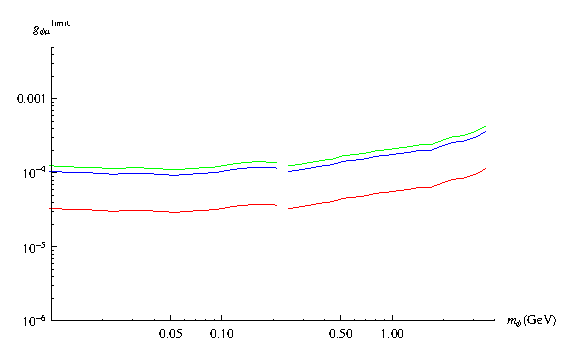
\includegraphics[width=0.6\textwidth]{Figures/limits/ee_all}
    \caption{Scalar limits from $e^+ e^-$ collisions at B-factories. Green, blue, and red represent \babar, \belle, and \belletwo respectively. Once the muon channel turns on, there is a large dip that is likely unphysical and may be due to poor background simulation in the case of a soft scalar.}
    \label{fig:ee_limits}
\end{figure}
